\section{METODOLOGI}

% Ubah konten-konten berikut sesuai dengan isi dari metodologi

\subsection{Metode yang digunakan}

Pada penelitian ini nantinya akan terdiri dari 2 langkah utama yaitu perancangan pada perangkat lunak (Softrware) dan perancangan pada perangkat keras (Hardware) :
%\begin{figure}[H]
%	\centering
%	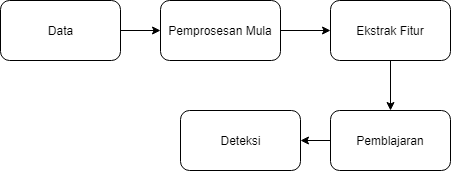
\includegraphics[width=\linewidth]{bab3/BlokDiagram}
%	\caption{Blok Diagram Penelitian}
%	\label{fig:blokdiagram}
%\end{figure}

\subsubsection{Perangkat Lunak}

\begin{figure}[!htbp]
	\centering
	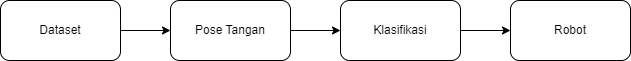
\includegraphics[width=1\linewidth]{gambar/gambar3.1}
	\caption{Blok Diagram Perangkat Lunak}
	\label{fig:gambar31}
\end{figure}

\subsubsubsection{Dataset}
Pada tahapan dataset disini akan dilakukan mulai dari pengambilan data-data yang disini nantinya akan berupa gambar/citra sampai dengan menyeleksi citra tersebut dan siap melanjutkan ke tahapan selanjutnya.

\begin{figure}[!htbp]
	\centering
	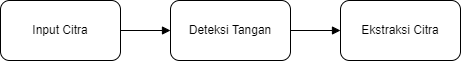
\includegraphics[width=0.7\linewidth]{gambar/Dataset.png}
	\caption{Blok Diagram Pembuatan Dataset}
	\label{fig:gambar32}
\end{figure}

\paragraph{Input Citra}
Pada dasarnya untuk mendeteksi suatu pose atau gerakan dari tangan membutuhkan untuk menemukan bagian tangan pada setiap Frame dan kemudian menganalisa pose atau gerakan tangan tersebut. Kamera digunakan untuk mendapatkan pose dari tangan pada setiap frame yang akan digunakan oleh user sebagai input untuk menentukan perintah. Dari input kamera ini yang nantinya akan digunakan untuk mendeteksi adanya tangan pada frame menggunakan Mediapipe.

\paragraph{Deteksi Tangan}
Mediapipe pada tangan memiliki 21 titik keypoint pada tangan. Setiap keypoint memiliki atribut posisi x, y, dan z. Data dari setiap titik yang nantinya akan diolah untuk menentukan gerakan dari tangan. Data koordinat dari setiap keypoint yang telah di dapatkan akan dilakukan normalisasi. Koordinat yang telah didapatkan merupakan koordinat dari setiap titik terhadap titik nol citra. Maka diperlukan perubahan dimana  koordinat setiap titik dirubah menjadi terhadap titik 0 keypoint. Jadi setiap ada perubahan posisi pada tangan masih dapat terukur posisinya terhadap titik 0 keypoint. Untuk jarak antar keypoint akan di scaling menggunakan jarak titik 0 ke titik 5 untuk menangani masalah dekat atau jauhnya tangan dari kamera. Untuk sudut pada tangan akan ada 3 titik dimana dianggap tidak bisa berotasi atau memilki sudut 0° yaitu pada titik 0, 5, dan 17. Dari titik - titik yang diketahui akan dihubungkan hingga berbentuk rangka dari tangan. Dari koordinat pada setiap titik tersebut akan dicari nilai terkecil terhadap sumbu x dan sumbu y pada citra. Dari nilai terkecil tersebut akan dibuatkan sebuah kotak untuk menandai bahwa yang didalam kotak tersebut adalah rangka tangan yang telah terdeteksi oleh mediapipe. 

\paragraph{Ekstraksi Citra}
Tangan yang telah terdeteksi oleh mediapipe dan telah terdapat rangkanya pada setiap frame akan disimpan untuk menjadi dataset. Citra yang disimpan akan ada 2 macam yaitu citra yang ditangkap oleh kamera dan terdapat ditangannya dan juga terdapat citra dengan latar berwarna hitam dengan rangka tangan dari mediapipe didalamnya. Citra berwana hitam sebelum disimpan akan dipotong sesuai luas dari kotak yang diambil dari koordinat terkecil dari 21 titik mediapipe. Ukuran dari citra yang telah dipotong akan diubah menjadi 256 {\textit{pixels}} secara vertikal dan 256 {\textit{pixels}} secara horizontal. Setelah ukuran citra hitam ini diubah menjadi 256 x 256 {\textit{pixels}}, citra tersebut akan disimpan dalam bentuk file png.

\subsubsubsection{Gestur Tangan}
Gestur tangan yang akan digunakan nantinya akan ada 5 getur yang akan sebagai simbol dari diam, maju, mundur, belok kanan, dan belok kiri. Diam akan disimbolkan dengan membuka telapak tangan serta meluruskan semua jari tangan. Maju akan disimbolkan dengan tangan mengepal 


\subsubsubsection{Classification}
Data yang sudah didapatkan nantinya akan di inputkan ke dalam perhitungan menggunakan machine learning. Data yang telah diinputkan nantinya akan dilabeli untuk ada diklasifikasikan dan digunakan untuk memberikan action selanjutnya. Dari hasil kalsifikasi nantinya akan disimpan sebagai model yang nantinya akan digunakan untuk mendeteksi citra yang akan datang

\subsubsubsection{Action}
Dari data yang telah di klasifikasikan dan sudah didapatkan gesturnya maka gestur tersebut akan diterjemahkan ke dalam suatu perintah untuk dapat menggerakkan mobil robot.

\subsubsection{Perangkat Keras}

\begin{figure}[!htbp]
	\centering
	\includegraphics[width=0.7\linewidth]{"gambar/gambar perangkat keras"}
	\caption{Blok Diagram Perangkat Keras}
	\label{fig:gambar33}
\end{figure}

\subsubsubsection{Laptop}
Laptop disini nantinya akan digunakan untuk menjalankan program perangkat lunak yang telah dikembangnkan untuk dapat menklasifikasikan tangan yang terdeteksi dan juga kamera yang terdapat pada laptop ini juga yang nantinya akan digunakan sebagai input gambar/citra.

\subsubsubsection{Bluetooth}
Hasil klasifikasi yang ada pada laptop akan dikirim ke mobil robot untuk dapat memberikannya perintah sesuia dari hasil klasifikasi. Menghubungkan laptop dan robot ini akan menggunakan modul \textit{bluetooth} yang akan dihubungkan dengan mobil robot dikarenakan mobil robot yang akan digunakan masih belum mempunyai modul \textit{bluetooth}. 

\subsubsubsection{Mobil Robot}
Pada bagian mobil robot ini terdapat beberapa komponen elektronik yang terpasang, diantaranya sebuatu mikrokontroller Arduino uno dan mikrokontroller Arduino nano , 2 buah .FC-03 L298N motor driver dual, modul charger Tp 4056, dan modul bluetooth HC-05. Komponen mekanik terdapat 4 buah roda, 4 buah gearbox motor, dan 1 buah chassis. \parencite*{JurnalElectroLuecat}

\subsection{Bahan dan peralatan yang digunakan}

\lipsum[13]
\lipsum[3]

\subsection{Urutan pelaksanaan penelitian}

% Ubah tabel berikut sesuai dengan isi dari rencana kerja
\newcommand{\w}{}
\newcommand{\G}{\cellcolor{gray}}
\begin{table}[h!]
  \begin{tabular}{|p{3.5cm}|c|c|c|c|c|c|c|c|c|c|c|c|c|c|c|c|}

    \hline
    \multirow{2}{*}{Kegiatan} & \multicolumn{16}{|c|}{Minggu} \\
    \cline{2-17} &
    1 & 2 & 3 & 4 & 5 & 6 & 7 & 8 & 9 & 10 & 11 & 12 & 13 & 14 & 15 & 16 \\
    \hline

    % Gunakan \G untuk mengisi sel dan \w untuk mengosongkan sel
    Pengambilan data &
    \G & \G & \G & \G & \w & \w & \w & \w & \w & \w & \w & \w & \w & \w & \w & \w \\
    \hline

    Pengolahan data &
    \w & \w & \w & \w & \G & \G & \G & \G & \w & \w & \w & \w & \w & \w & \w & \w \\
    \hline

    Analisa data &
    \w & \w & \w & \w & \w & \w & \w & \w & \G & \G & \G & \G & \w & \w & \w & \w \\
    \hline

    Evaluasi penelitian &
    \w & \w & \w & \w & \w & \w & \w & \w & \w & \w & \w & \w & \G & \G & \G & \G \\
    \hline

  \end{tabular}
\end{table}
